\documentclass[a4paper,12pt]{article}

\title{Chapter 4. Interacting Fields and Feynman Diagrams\\
4.6 Computing S-Matrix Elements from Feynman Diagrams}
\date{各種SNS\\
    X (旧 Twitter): \href{https://x.com/miya_max_study}{@miya\_max\_study}\\
    Instagram : \href{https://www.instagram.com/daily_life_of_miya/}{@daily\_life\_of\_miya}\\
    YouTube : \href{https://www.youtube.com/@miya-max-active}{@miya-max-active}
    }
\author{Max Miyazaki}

\usepackage{amsmath}
\usepackage{amssymb}
\usepackage{ascmac}
\usepackage{amsthm}
\usepackage{amsfonts}
\usepackage{enumitem}
\usepackage{color}
\usepackage[dvipdfmx]{graphicx}
\usepackage{float}
\usepackage{bm}
\usepackage{here}
\usepackage{simpler-wick}

\usepackage{abstract}
\usepackage{tikz}
\usetikzlibrary{shapes.geometric, arrows.meta, positioning}
\usepackage{indentfirst}
\usepackage[utf8]{inputenc}
\usepackage{fix-cm}
\usepackage{wrapfig}
\pagenumbering{arabic}
\usepackage{url}
\usepackage{xcolor}
\usepackage[most]{tcolorbox}
\usepackage{framed}
\usepackage[dvipdfmx]{hyperref}
\hypersetup{
 setpagesize=false,
 bookmarksnumbered=true,
 colorlinks=true,
 linkcolor=blue
}

% Define braket-like commands
\newcommand{\bra}[1]{\left\langle #1\right|}
\newcommand{\ket}[1]{\left|#1\right\rangle}
\newcommand{\braket}[2]{\left\langle #1\middle|#2\right\rangle}
\newcommand{\brakets}[3]{\left\langle #1\middle| #2 \middle|#3 \right\rangle}

\renewcommand{\arraystretch}{2.1}


\setlength{\textwidth}{16cm}
\setlength{\textheight}{25cm}
\setlength{\oddsidemargin}{0cm}
\setlength{\evensidemargin}{0cm}
\setlength{\topmargin}{-2cm}

\begin{document}
\maketitle

\vspace{1cm}
\begin{abstract}
    このノートはPeskin\&Schroederの``An Introduction to Quantum Field Theory''の第4章の5節をまとめたものである. 要点や個人的な追記, 計算ノート的なまとめを行っているが, それらはすべて原書の内容を出発点としている. 参考程度に使っていただきたいが, このノートは私の勉強ノートであり, そのままの内容をそのまま鵜呑みにすると間違った理解を招く可能性があることをご了承ください. ぜひ原著を手に取り, その内容をご自身で確認していただくことを推奨します. てへぺろ v$({\hat{\cdot}_\partial \hat{\cdot}})$v
\end{abstract}
    
    

\newpage
\color{blue}
\section*{概要}

\begin{itemize}
  \item \textbf{目標}
  \begin{itemize}
    \item 相互作用場の摂動論を, 時空的過程 (因果律) として視覚化できる形式で発展させる.
    \item まず二点相関関数(グリーン関数)の計算から始める.
  \end{itemize}

  \item \textbf{二点相関関数の定義}
  \begin{itemize}
    \item $\phi^4$ 理論において基底状態 $\lvert \Omega \rangle$ の二点相関関数を考える:
    \begin{equation*}
      \langle \Omega | T\{\phi(x)\phi(y)\} | \Omega \rangle .
    \end{equation*}
    \item 自由理論ではこれはファインマン伝播子に一致する.
  \end{itemize}

  \item \textbf{相互作用の導入}
  \begin{itemize}
    \item Hamiltonian を $H = H_0 + H_{\text{int}}$ に分け, 相互作用を摂動として扱う.
    \item 相互作用表示を用いて, 自由場 $\phi_I$ を基礎に展開する.
  \end{itemize}

  \item \textbf{時間発展演算子 $U(t,t_0)$}
  \begin{itemize}
    \item ハイゼンベルク場 $\phi$ は
    \begin{equation*}
      \phi(t,\mathbf{x}) = U^\dagger(t,t_0)\phi_I(t,\mathbf{x})U(t,t_0)
    \end{equation*}
    で表される.
    \item $U(t,t_0)$ は Dyson 展開で表現される:
    \begin{equation*}
      U(t,t_0) = T \exp\left[ -i\int_{t_0}^t dt' \, H_I(t') \right].
    \end{equation*}
  \end{itemize}

  \item \textbf{基底状態 $\lvert \Omega \rangle$ の構成}
  \begin{itemize}
    \item 相互作用を含む基底状態は, 自由理論の真空 $\lvert 0 \rangle$ を時間発展させることで得られる.
    \item 大きな $T$ の極限をとることで, 基底状態 $n=0$ の項のみが残る.
  \end{itemize}

  \item \textbf{二点相関関数の最終式}
  \begin{itemize}
    \item 相関関数は真空期待値で表される:
    \begin{equation*}
      \langle \Omega | T\{\phi(x)\phi(y)\} | \Omega \rangle
      = \lim_{T \to \infty (1-i\epsilon)}
      \frac{\langle 0 | T \{ \phi_I(x)\phi_I(y)\exp[-i\int_{-T}^T dt\, H_I(t)] \} | 0 \rangle}
      {\langle 0 | T \{ \exp[-i\int_{-T}^T dt\, H_I(t)] \} | 0 \rangle}.
    \end{equation*}
    \item これは \textbf{相互作用表示における Wick の定理} の基礎となる.
  \end{itemize}

  \item \textbf{意義}
  \begin{itemize}
    \item 時間順序積を導入することで, すべての相関関数を1つの $T$-積の中にまとめられる.
    \item 高次相関関数にも容易に拡張可能.
    \item 実際の計算では指数をテイラー展開し, 必要な次数まで項を残せば十分である.
  \end{itemize}

\end{itemize}
\newpage
\color{black}
\section*{4.6 Computing S-Matrix Elements from Feynman Diagrams}

我々はこれまでに断面積と崩壊率の公式を導出した。  
残る課題は、相互作用する場の様々な過程に対して $\mathcal{M}$ を計算する方法を見つけることである。  
次節以降では、ファインマン図を用いて $\mathcal{M}$ を表現する公式を記す。  

S行列の定義 (4.71) を思い出すと:

\begin{equation}
\langle p_1 p_2 \cdots | S | k_A k_B \rangle
= \lim_{T\to\infty} \langle p_1 p_2 \cdots | e^{-iH(2T)} | k_A k_B \rangle.
\tag{4.87}
\end{equation}

この量を計算するために、我々は外部1粒子状態を、非摂動論の基底である $|\Omega\rangle$ の対応物に置き換える。  
式 (4.27) における $|\Omega\rangle$ は

\[
|\Omega\rangle = \lim_{T\to\infty(1-i\epsilon)} 
(e^{-iE_0T} \langle \Omega|0\rangle )^{-1} e^{-iHT}|0\rangle
\]

で与えられていた。  

これと同様に、今度は

\begin{equation}
|k_A k_B\rangle \propto 
\lim_{T\to\infty(1-i\epsilon)} e^{-iHT} |k_A k_B\rangle_0
\tag{4.88}
\end{equation}

という関係式を見つけたい。そのような関係を見出すのは容易ではない。式(4.27)では、真空が絶対的な最低エネルギー状態であるという事実を用いた。ここでは、初期粒子と最終粒子が十分に分離した外部状態が、あらかじめ決められた非零の運動量値と整合する最低エネルギーを持つという、はるかに弱い主張しか利用できない。

この公式 (4.88) が正当化されれば、(4.87) の右辺を書き換えて次のようにできる:

\begin{equation}
\lim_{T \to \infty(1-i\epsilon)} \langle p_1 \cdots p_n| e^{-iH(2T)} |p_A p_B\rangle_0
\propto \lim_{T \to \infty(1-i\epsilon)} 
\langle p_1 \cdots p_n| T\!\left(\exp\!\left[-i \int_{-T}^{T} dt\, H_I(t)\right]\right)|p_A p_B\rangle_0.
\tag{4.89}
\end{equation}

---

真空期待値を評価する際には、自由真空と相互作用真空の間の比例因子が最終式 (4.31) で打ち消されていた。  
現在の場合、その因子はさらに厄介であり、ここでは全く書き下していない。  
我々は同様の劇的な相殺がここでも起こることを期待するのみである。  

実際にそうした相殺が生じるとしても、我々の現在のアプローチからその結論を厳密に導くことは容易ではない。  

いずれにせよ、実用的には無視できる小さな修正を加えて、$S$ 行列の非自明な部分に対する公式は次の形に簡約される:

\begin{equation}
\langle p_1 \cdots p_n| iT | p_A p_B\rangle
= \lim_{T \to \infty(1-i\epsilon)} 
\langle p_1 \cdots p_n| T\!\left(\exp\!\left[-i \int_{-T}^{T} dt\, H_I(t)\right]\right) |p_A p_B\rangle_0^{\text{connected, amputated}}.
\tag{4.90}
\end{equation}

---

まず、式 (4.90) の行列要素をファインマン図の和として表す方法を学ぼう。  
具体例として、$\phi^4$ 理論における最初のいくつかの項を、最終状態に二粒子をもつ場合に評価する。  

最初の項は:

\begin{align}
\langle p_1 p_2| p_A p_B\rangle_0
&= \sqrt{2E_1 2E_2 2E_A 2E_B} \, \langle 0| a_{p_1} a_{p_2} a_{p_A}^\dagger a_{p_B}^\dagger |0\rangle \\
&= 2E_A 2E_B (2\pi)^6 \Big[ \delta^{(3)}(\mathbf{p}_A-\mathbf{p}_1)\delta^{(3)}(\mathbf{p}_B-\mathbf{p}_2)
+ \delta^{(3)}(\mathbf{p}_A-\mathbf{p}_2)\delta^{(3)}(\mathbf{p}_B-\mathbf{p}_1)\Big].
\tag{4.91}
\end{align}

デルタ関数は最終状態を初期状態と同一にする。したがってこの項は $S=1+iT$ の「1」の部分であり、散乱行列要素 $\mathcal{M}$ には寄与せず、以下の図で示せる:

\begin{figure}[H]
    \centering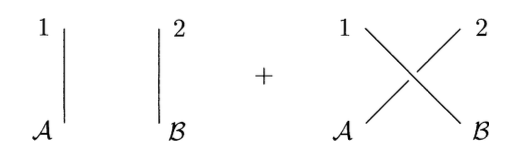
\includegraphics[width=0.6\textwidth]{figures/4.91a.png}
\end{figure}

次の項は:

\begin{align}
\langle p_1 p_2| T\!\left(-\frac{i\lambda}{4!} \int d^4x \, \phi_I^4(x)\right) |p_A p_B\rangle_0
&= \langle p_1 p_2| N\!\left(-\frac{i\lambda}{4!} \int d^4x \, \phi_I^4(x) + \text{収縮項}\right)|p_A p_B\rangle_0.
\tag{4.92}
\end{align}

---

ウィックの定理を用いると、外部状態が真空でないため完全に縮約されない項も寄与を持ちうる。  
例えば、$\phi_I(x)$ の消滅演算子を用いて初期状態粒子を消去したり、生成演算子を用いて最終状態粒子を生成することで寄与が生じる。  

例えば、

\begin{equation}
\phi_I^\dagger(x)|p\rangle_0
= \int \frac{d^3k}{(2\pi)^3} \frac{1}{\sqrt{2E_k}} a_k^\dagger e^{-ik\cdot x} \sqrt{2E_p} (2\pi)^3 \delta^{(3)}(\mathbf{k}-\mathbf{p})|0\rangle
= e^{-ip\cdot x}|0\rangle.
\tag{4.93}
\end{equation}

---

したがって、外部状態をもつ場の演算子を次のように定義するのが自然である:

\begin{equation}
\phi_I(x)|p\rangle = e^{-ip\cdot x}|0\rangle, 
\qquad
\langle p|\phi_I(x) = \langle 0| e^{+ip\cdot x}.
\tag{4.94}
\end{equation}

---

$S$ 行列要素を評価するためには、このような寄与をすべて書き下し、$\phi_I$ 演算子の全ての縮約と外部状態の運動量を考慮すればよい。  

例えば (4.92) を評価するために、$N$ 積は次の項を含む:

\begin{equation}
\wick{\c1 \phi \c1 \phi \c2 \phi \c2 \phi}, \quad
\wick{\c1 \phi \c2 \phi \c1 \phi \c2 \phi}, \quad
\wick{\c1 \phi \c2 \phi \c2 \phi \c1 \phi}.
\tag{4.95}
\end{equation}

最後の項では、すべての演算子が互いに完全に縮約されている。








\end{document}
